\documentclass{article}

\usepackage{mhchem} % Package for chemical equation typesetting
\usepackage{siunitx} % Provides the \SI{}{} command for typesetting SI units
\usepackage{pdfsync}
\usepackage[dutch]{babel}
\usepackage{fullpage}
\usepackage{amsmath}
\usepackage[table]{xcolor}
\usepackage{multirow}
\usepackage{graphicx}
\usepackage{circuitikz}
\usepackage{caption}
\usepackage{subcaption}
\usepackage{float}
\usepackage{verbatim}
\usepackage{eso-pic}
\usepackage[toc,page]{appendix}
\usepackage[linkbordercolor={white}]{hyperref}
\usepackage{nameref}
\usepackage{listings}
\usepackage{mcode}
\usepackage{graphicx} % Required for the inclusion of images

\setlength\parindent{0pt} % Removes all indentation from paragraphs

\renewcommand{\labelenumi}{\alph{enumi}.} % Make numbering in the enumerate environment by letter rather than number (e.g. section 6)

%\usepackage{times} % Uncomment to use the Times New Roman font

%----------------------------------------------------------------------------------------
%	DOCUMENT INFORMATION
%----------------------------------------------------------------------------------------

\title{Report Lab Assignment \\ Running x264 on Host Processor\\ Extracting and Accelerating Kernel on Co-processor} % Title

\author{Imara \textsc{Speek} (1506374)\\ Aimee \textsc{Ferouge} (4014030)} % Author name

\date{\today} % Date for the report

\begin{document}

\maketitle % Insert the title, author and date

\begin{center}
\begin{tabular}{l r}
Date Performed: & October, 2013 \\ % Date the experiment was performed
Instructor: & Ir. A. Brandon % Instructor/supervisor
\end{tabular}
\end{center}

 \begin{abstract}
 10 lines of Abstract text
 \end{abstract}

%----------------------------------------------------------------------------------------
%	Lijst van wat er nog moet gebeuren
%----------------------------------------------------------------------------------------

\section{Wat moet er nog gebeuren}
\begin{itemize}
\item debuggen van de rovex uitleggen met nep pixels en bewijs van werking
\item Stride en manier van het schrijven naar het geheugen uitleggen
\item Gebruik van lseek uitleggen
\item uitleg van de kernel functie met plaatjes
\item communicatie van pvex en microblaze
\item big or little endiannes, en aanpak in code
\item speedup \& theoretical calculation speedup
\item results of additional assignment and if more time which we would have chosen
\end{itemize}

%----------------------------------------------------------------------------------------
%	Introduction
%----------------------------------------------------------------------------------------

% Introduction

\section*{Introduction}

*Introduction* \cite{fpga} blabla \cite{why}

 
%----------------------------------------------------------------------------------------
%	De rest
%----------------------------------------------------------------------------------------

% -- Approach ---------------------------------------
\section{Approach}
\label{sec:approach}
%Our extracted kernel can be found in appendix \ref{sec:satd}. 
The kernel can run in the $\rho$-VEX by putting the \mcode{bytecode} generated by the \mcode{makefile} into the instruction memory of the $\rho$-VEX and placing all required data in its data memory dynamically. By executing \mcode{make byte-} command two files are created:
\begin{itemize}
	\item \mcode{bytecode}, containing all the intstructions to be executed by the $\rho$-VEX
	\item \mcode{bytedata}, containing the pixels of the input stream
\end{itemize}

In order to make the extracted kernel qualified for compilation and execution, a few things have to be altered. First, the new file has to be recognized by the \mcode{makefile} in the rovex-examples directory. Second, some type definitions have to be made. Originally, \mcode{pixel\_satd\_8x4} resides in the \mcode{pixel.c} file of the x264 application. When extracting this kernel, all prior knowledge is lost and has to be defined again. Then, in order to make the kernel compile and run on the $\rho$-VEX, the development board has to be reset and started. \mcode{Bytecode} has to be written to the instruction memory (\mcode{rvex-imemory}) and \mcode{bytedata} to the data memory (\mcode{rvex-dmemory}). Finally, the calculated result should be returned to the host. Figure \ref{fig:rvex-dmem} shows the $\rho$-VEX memory layout for our kernel.
% --- dmem of the ROVEX ----------------------------------
\begin{figure}[htb]%
\centering
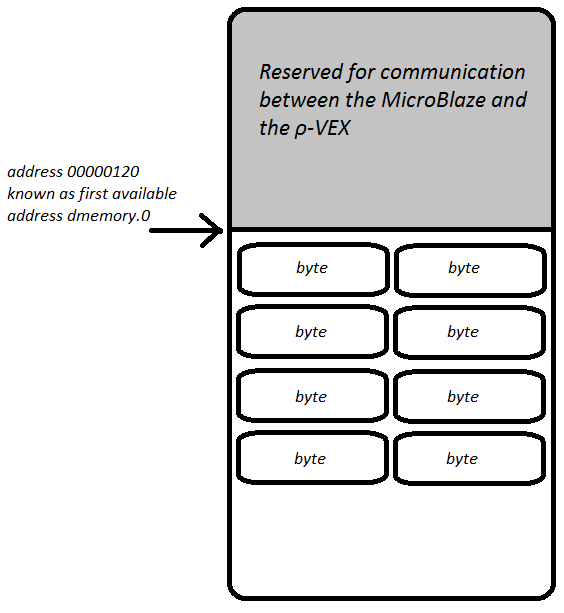
\includegraphics[height=200px]{Pictures/dmem_rvex}%
\caption{Memory layout of the $\rho$-VEX}%
\label{fig:rvex-dmem}%
\end{figure}

\subsection{Adjusting the \mcode{makefile}}
We added the kernel to the \mcode{EXECUTABLES} defined in the \mcode{makefile}. Other files defined here can be removed since we will not need them for our application. An important issue is the difference between logical memory and physical memory. While the first address of a logical memory is obviously address '0', the physical memory can have the first part of the register being occupied (e.g. by the operating system). For the $\rho$-VEX, the first address which is allowed to be written to is 0x120. Thus, when writing the result of the kernel to the logical address '0', it is  actually writing to the physical address '120' of the data memory. %This can be done using \mcode{\_\_DATA\_START} to indicate the start address.

Despite the fact that this is a rather simplistic operation, it took us some struggling to properly distinguish these address spaces. For example, we were told by the TA to remove the \mcode{autoinline} flag which resulted in a lot of wrong hexdumps. Also, the introduced fix discussed in \ref{sec:fix} caused some problems that took us until the end of the second week to resolve.

\subsection{Constraints of the $\rho$-VEX}
Using the $\rho$-VEX as a co-processor comes with some limitations. First, the $\rho$-VEX supports a very old and basic C compiler, so using \mcode{printf} statements to find bugs in the extracted kernel file is not possible. Everytime the application is being run concurrently on the $\rho$-VEX, the status is being inspected by placing \mcode{printf} statements in the \mcode{pixel.c} file, the origin of the kernel. Also, the $\rho$-VEX is very strict in the order of variable declarations and initialization. One of our bugs involved \mcode{int i} being declared and initialized, followed by a declaration of \mcode{int result}. This is not supported by the $\rho$-VEX, since it wants to have \mcode{int i, result;} both to be declared first, before initializing \mcode{i = 4;}.

When running an extracted kernel on the $\rho$-VEX, the kernel is unable to obtain information from previous code. Consequently, all parameters have to be re-defined. Table \ref{tab:typedef} shows all required type definitions.

% -- Type Definitions ---------------------------------------
\begin{table}[htb]%
\begin{tabular}{lll}
	\bf{Parameter} 					& \bf{Type definition} 					& \bf{Motivation}\\ \cline{1-3}
	\mcode{intptr\_t}				&	\mcode{unsigned int}					& This parameter represents the stride, which cannot be $<$0\\
	\mcode{pixel}						& \mcode{unsigned char}					&	Pixels are made out of bytes, which have 8 bits (like a \mcode{char})\\
	\mcode{sum\_t}					&	\mcode{short int}							& Same type definition as in the source code (16 bits)\\
	\mcode{sum2\_t}					& \mcode{long int}							& Same type definition as in the source code (32 bits)\\
	\mcode{BIT\_DEPTH}			& defined as 8									& Also in the source code, plus the kernel handles pixels (bytes)\\
	\mcode{BIT\_PER\_SUM}		&	(8 * \mcode{sizeof(sum\_t)})	& Also predefined as in the source code, being 16 \\
\end{tabular}
\caption{Type definitions in the extracted kernel file.}
\label{tab:typedef}
\end{table}


\subsection{Communication between the MicroBlaze and the $\rho$-VEX}

In order to delegate the \mcode{pixel\_satd\_8x4} kernel from the MicroBlaze to the $\rho$-VEX, both the environments need to communicate with each other. When executing the x264 application, the MicroBlaze has to load the instructions of the extracted kernel into the instruction memory of the $\rho$-VEX and the data (for which the SATD has to be evaluated) into the data memory. This is when the source code of x264 becomes involved. The \mcode{pixel\_satd\_8x4 kernel}, which is residing in the \mcode{pixel.c} file of the application, needs to be adjusted. Instead of calculating the SATD itself, it should send the instructions and input data to the $\rho$-VEX. The commands \mcode{open()}, \mcode{close()}, \mcode{read()} and \mcode{write()} are therefor added to the \mcode{pixel.c} file of the x264 application. These pixels are written at physical address 120, the first address on the $\rho$-VEX that is not set apart for communication between the driver and the $\rho$-VEX, defined as address '0'. To be sure that the data is always written to the same location we use the \mcode{lseek()} function to specify the start location of data as 0x00 from the \mcode{SEEK_SET}, or the beginning of the file. 

To control the $\rho$-VEX from the x264 application, the control registers can be written too. By writing \mcode{'2'} to the control registers, the $\rho$-VEX is being reset. It can then be started by writing \mcode{'1'} to the register, telling the $\rho$-VEX to start running the instructions available in the instruction memory, calculating the SATD of the two pixels. While calculating, the status of the $\rho$-VEX can be checked in a \mcode{while}-loop by reading the status variable of the status memory (\mcode{rvex-smemory}). When the kernel is finished, the result can be read from the data memory. See also \mcode{pixel.c}.

\subsection{Result Hyphothesis}

By having the computational intensive kernel being run concurrently on a co-processor, one would expect an overal speedup of the application. A problem is, however, that the \mcode{bytecode} and the data have to be sent to the $\rho$-VEX every time the kernel is being called. The data contains two new pixels of which the SATD has to be calculated, whereas \mcode{bytecode} holds the kernel instructions. Because of this constant data traffic between the MicroBlaze and the $\rho$-VEX we don't expect the intended speed up to be achieved.

The reason that \mcode{bytecode} has to be sent every time the kernel is called, is that the three available FPGAs are shared among a lot of students. When running their application concurrently, the instruction memory is constantly being overwritten by another group. If there was a one-to-one setup, \mcode{bytecode} could have to been placed in \mcode{main.c}, written tot the \mcode{imemory} of the $\rho$-VEX only once when starting the application. 



% -- Implementation ---------------------------------------

\section{Implementation}

The approach described in the previous section wasn't implemented in a day, obviously. This section will cover some difficulties that came along during the lab.

\subsection{The Fix}
Halfway the lab, a fix was introduced. Setting the physical start addres to 0x120 was now done and did not have to be passed on using \mcode{\_\_DATA\_START}. In order to make the $\rho$-VEX read the pixels in the data memory correct a pointer to the first logical address 0 would be enough.

Unfortunately, this caused us problems for weeks. Since we wanted to let the original x264 file unaltered, we copied the folder and created a new application. The folder was called 'lab2', with the \mcode{pixel.c} file called \mcode{microlab2.c}. The \mcode{lab2.c} file containing the extracted kernel was in the rovex-examples folder because of the \mcode{makefile}, that was also residing there. Now, the fix was only applicable to the original x264 folder, so we still had to deal with the stride issue.

When we found out about this fix, we adjusted the original x264 folder. We commented out the source code of \mcode{pixel_satd_8x4} and put our MicroBlaze kernel code instead. To check whether the pixels were sent to $\rho$-VEX data memory correctly, we pre-defined two pixels in \mcode{pixel.c} to be written to \mcode{rvex-dmemory}. This way, we could have certain expectations when doing a \mcode{hexdump} to examine the registers. Our testpixels are shows in figure \ref{fig:test}.

\begin{figure}
	\centering
	\begin{subfigure} [h] {0.5\textwidth}
		\centering
		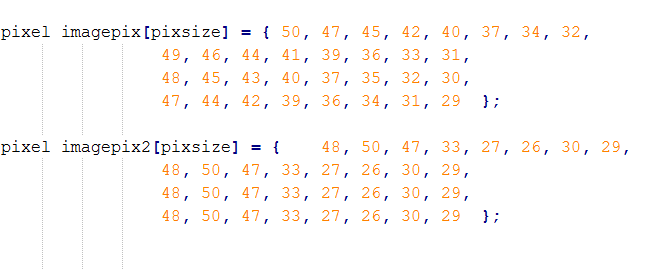
\includegraphics[width=150px]{Pictures/testpixels}
		\caption{Test pixels defined in \mcode{pixel.c}}
		\label{fig:test}
	\end{subfigure}
	\quad
	\begin{subfigure} [h] {0.5\textwidth}
		\centering
		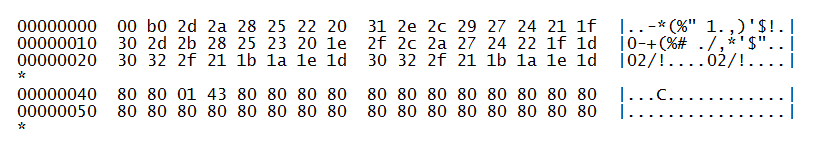
\includegraphics[width=150px]{Pictures/hextest}
		\caption{Hexdump of the testpixels (first two bytes incorrect)}
		\label{fig:testhex}
	\end{subfigure}
	\quad
\caption{Commands for reading from and writing to the $\rho$-VEX}%
\label{}%
\end{figure}


\subsection{Order of Variable Initialization}

After moving our code to the original x264 code and creating test pixels to be used for SATD calculation, a dump of the $\rho$-VEX data memory can been seen in figure \ref{fig:testhex}. As you can see, the first two byte are not matching. At first, we thought this could be because of the fact that another group was running their application at the same FPGA concurrently. However, the value of these bytes remained the same during several runs. 

This unwanted write was caused by the initialization of the \mcode{sum} variable, that has type \mcode{short int} and was stored in the data memory before the pixel. When \mcode{pixel_satd_8x4} tried to find the pixels, it found \mcode{sum} instead of the pixels, causing the program to get stuck in a loop. When changes \mcode{sum} to not being initiazlied, \mcode{datamem} containing the pixels had the first spot at address 120.

\subsection{Endianness}
The MicroBlaze and the $\rho$-VEX understand basic operations like \mcode{open()}, \mcode{close()}, \mcode{read()} and \mcode{write()}. However, they differ in Endiannes. $\rho$-VEX operates in Little Endian, meaning the bytes are read from right to left, as seen in figure \ref{fig:little}. MicroBlaze, on the other hand, operates in Big Endian and thus reads the bytes from left to right (see figure \ref{fig:big}). This becomes an issue when reading the \mcode{result} variable from the data memory, as we will get the bytes in reversed order. This problem is solved by manually reversing the order of the \mcode{result} bytes, realized by the piece of code in figure \ref{fig:swap}.

\begin{figure}
	\centering
	\begin{subfigure} [h] {0.5\textwidth}
		\centering
		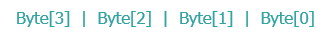
\includegraphics[width=150px]{Pictures/little}
		\caption{Little Endian}}
		\label{fig:little}
	\end{subfigure}
	\quad
	\begin{subfigure} [h] {0.5\textwidth}
		\centering
		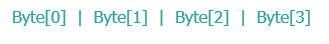
\includegraphics[width=150px]{Pictures/big}
		\caption{Big Endian}
		\label{fig:big}
	\end{subfigure}
	\quad
	\begin{subfigure} [h] {0.5\textwidth}
		\centering
		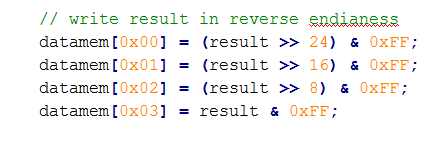
\includegraphics[width=150px]{Pictures/byteswap}
		\caption{Reversing the order of bytes}
		\label{fig:swap}
	\end{subfigure}
\caption{Different reading direction due to Endianness}%
\label{}%
\end{figure}

\subsection{Setting pointer to address 0 using \mcode{lseek}}

When writing pixels to the data memory of the $\rho$-VEX, it is important to know exactly where they end up. This situation can be solved by using \mcode{lseek}, a system call that is used to change the location of the read/write pointer of a file descriptor. When ordering \mcode{lseek(data, 0, SEEK_SET)}, the pointer in the $\rho$-VEX moves to the address that is the start address from his point of view (thus, physical address 0x120). We first made a mistake by putting 0x120 as \mcode{lseek} parameter, which gives an error since the MicroBlaze can not see into the physical address of the $\rho$-VEX. Translating the logical address 0 to the physical address 0x120 is done by the linker and is not of our concern.



\appendix
\section{Extracted kernels \mcode{pixel_satd_8x4} and \mcode{pixel_satd_4x4}}
\label{sec:satd}

\lstinputlisting{kernel.c}



%----------------------------------------------------------------------------------------
%	BIBLIOGRAPHY
%----------------------------------------------------------------------------------------
%
%\bibliographystyle{unsrt}
%
%\bibliography{sample}
%
%----------------------------------------------------------------------------------------


\end{document}